\documentclass[english]{article}
\usepackage{graphicx}
\usepackage{amsmath}
\usepackage{hyperref}
\usepackage{setspace}
\usepackage{apacite}
\usepackage{hyperref}
\usepackage{natbib}
\usepackage{pxfonts}
\usepackage[utf8]{inputenc}
\usepackage[left=1in,right=1in,top=1in,bottom=1in]{geometry}
\usepackage[left]{lineno}
\usepackage{soul}
\linenumbers


\title{High-order cognition is supported by complex but compressible brain activity patterns} 

\author{Lucy L. W. Owen\textsuperscript{1, 2}, and Jeremy R. Manning\textsuperscript{1,
*}\\\textsuperscript{1}Department of Psychological and Brain Sciences,\\Dartmouth College,
Hanover, NH\\[0.1cm]\textsuperscript{2}Carney Institute for Brain Sciences,\\Brown University,
Providence, RI\\[0.1cm] \textsuperscript{*}Address correspondence to
jeremy.r.manning@dartmouth.edu}

\begin{document}
\maketitle


\begin{abstract} 

We applied dimensionality reduction algorithms and pattern classifiers to
functional neuroimaging data collected as participants listened to a story,
temporally scrambled versions of the story, or underwent a resting state
scanning session. These experimental conditions were intended to require
different depths of processing and insprire different levels of engagement. We
considered two primary aspects of the data. First, we treated the number of
features (components) required to achieve a threshold decoding accuracy as a
proxy for the ``compressibility'' of the neural patterns (where fewer
components indicate higher compressibility). Second, we treated the maximum
achievable decoding accuracy across participants as an indicator of the
``stability'' of the recorded patterns. Overall, we found that neural patterns
recorded as participants listened to the intact story required fewer features
to achieve comparable classification accuracy to the other experimental
conditions. However, the peak decoding accuracy (achievable with more features)
was also highest during intact story listening. Taken together, our work
suggests that our brain networks flexibly reconfigure according to ongoing task
demands, and that the activity patterns associated with higher-order cognition
and high engagement are both more complex and more compressible than the
activity patterns associated with lower-order tasks and lower levels of
engagement.

\end{abstract}

\doublespacing

\section*{Introduction}

Large-scale networks, including the human brain, may be conceptualized as
occupying one or more positions along on a continuum. At one extreme, every
node is fully independent of every other node. At the other extreme, all nodes
behave identically. Each extreme optimizes key properties of how the network
functions. When every node is independent, the network is maximally
\textit{expressive}: if we define the network's ``state'' as the activity
pattern across its nodes, then every state is equally reachable by a network
with fully independent nodes. On the other hand, a network of identically
behaved nodes optimizes \textit{robustness}: any subset of nodes may be removed
from the network without any loss of function or expressive power, as long as
any single node remains. Presumably, most natural systems tend to occupy
positions between these extremes. We wondered: might the human brain
reconfigure itself to be more flexible or more robust according to ongoing
demands? In other words, might the brain reconfigure its connections or
behaviors under different circumstances to change its position along this
continuum?

% compression (redundancy) vs. complexity -- appear to balance each other, butnot necessarily. 

Closely related to the above notions of expressiveness versus robustness are
measures of how much \textit{information} is contained in a given signal or
pattern, and how \textit{redundant} a signal is~\citep{Shan48}. Formally,
information is defined as the amount of uncertainty about a given variables'
outcomes (i.e., entropy), measured in \textit{bits}, or the optimal number of
yes/no questions needed to reduce uncertainty about the variable's outcomes to
zero. Highly complex systems with many degrees of freedom (i.e., high
flexibility and expressiveness), are more information-rich than simpler or more
constrained systems. The redundancy of a signal denotes the difference how
expressive the signal \textit{could} be (i.e., proportional to the number of
unique states or symbols used to transmit the signal) and the actual
information rate (i.e., the entropy of each individual state or symbol). If a
brain network's nodes are fully independent, then the number of bits required
to express a single activity pattern is proportional to the number of nodes.
The network would also be minimally redundant, since the status of every node
would be needed to fully express a single brain activity pattern. If a brain
network's nodes are fully coupled and identical, then the number of bits
required to express a single activity pattern is proportional to the number of
unique states or values any individual node can take on. Such a network would
be highly redundant, since knowing any individual node's state would be
sufficient to recover the full-brain activity pattern. Highly redundant systems
are also robust, since there is little information loss from losing any given
observation.

We take as a given that brain activity is highly flexible: our brains can
exhibit nearly infinite activity patterns. This flexibility implies that our
brains activity patterns are highly information rich. However, brain activity
patterns are also highly structured. For example, full-brain correlation
matrices are stable within~\citep{FinnEtal15, FinnEtal17, GratEtal18} and
across~\citep{YeoEtal11, GlerEtal12, GratEtal18, ColeEtal14} individuals. This
stability suggests that our brains' activity patterns are at least partially
constrained, for example by anatomical, external, or internal factors.
Constraints on brain activity that limit its flexibility decrease
expressiveness (i.e., its information rate). However, constraints on brain
activity also increase its robustness to noise (e.g., ``missing'' or corrupted
signals may be partially recovered). For example, recent work has shown that
full-brain activity patterns may be reliably recovered from only a relatively
small number of implanted electrodes~\citep{OwenEtal20, ScanEtal21}. This
robustness property suggests that the relevant signal (e.g., underlying factors
that have some influence over brain activity patterns) are compressible.

To the extent that brain activity patterns contain rich task-relevant
information, we should be able to use the activity patterns to accurately
differentiate between different aspects of the task~\citep[e.g., using pattern
classifiers;][]{NormEtal06b}. For example, prior work has shown a direct
correspondence between classification accuracy and the information content of a
signal~\citep{Alva02}. To the extent that brain activity patterns are
compressible, we should be able to generate simplified (e.g., lower
dimensional) representations of the data while still preserving the relevant or
important aspects of the original signal. In general, information content and
compressibility are related but are partially dissociable
(Fig.~\ref{fig:information-compression}).

\begin{figure}[tp]

\centering
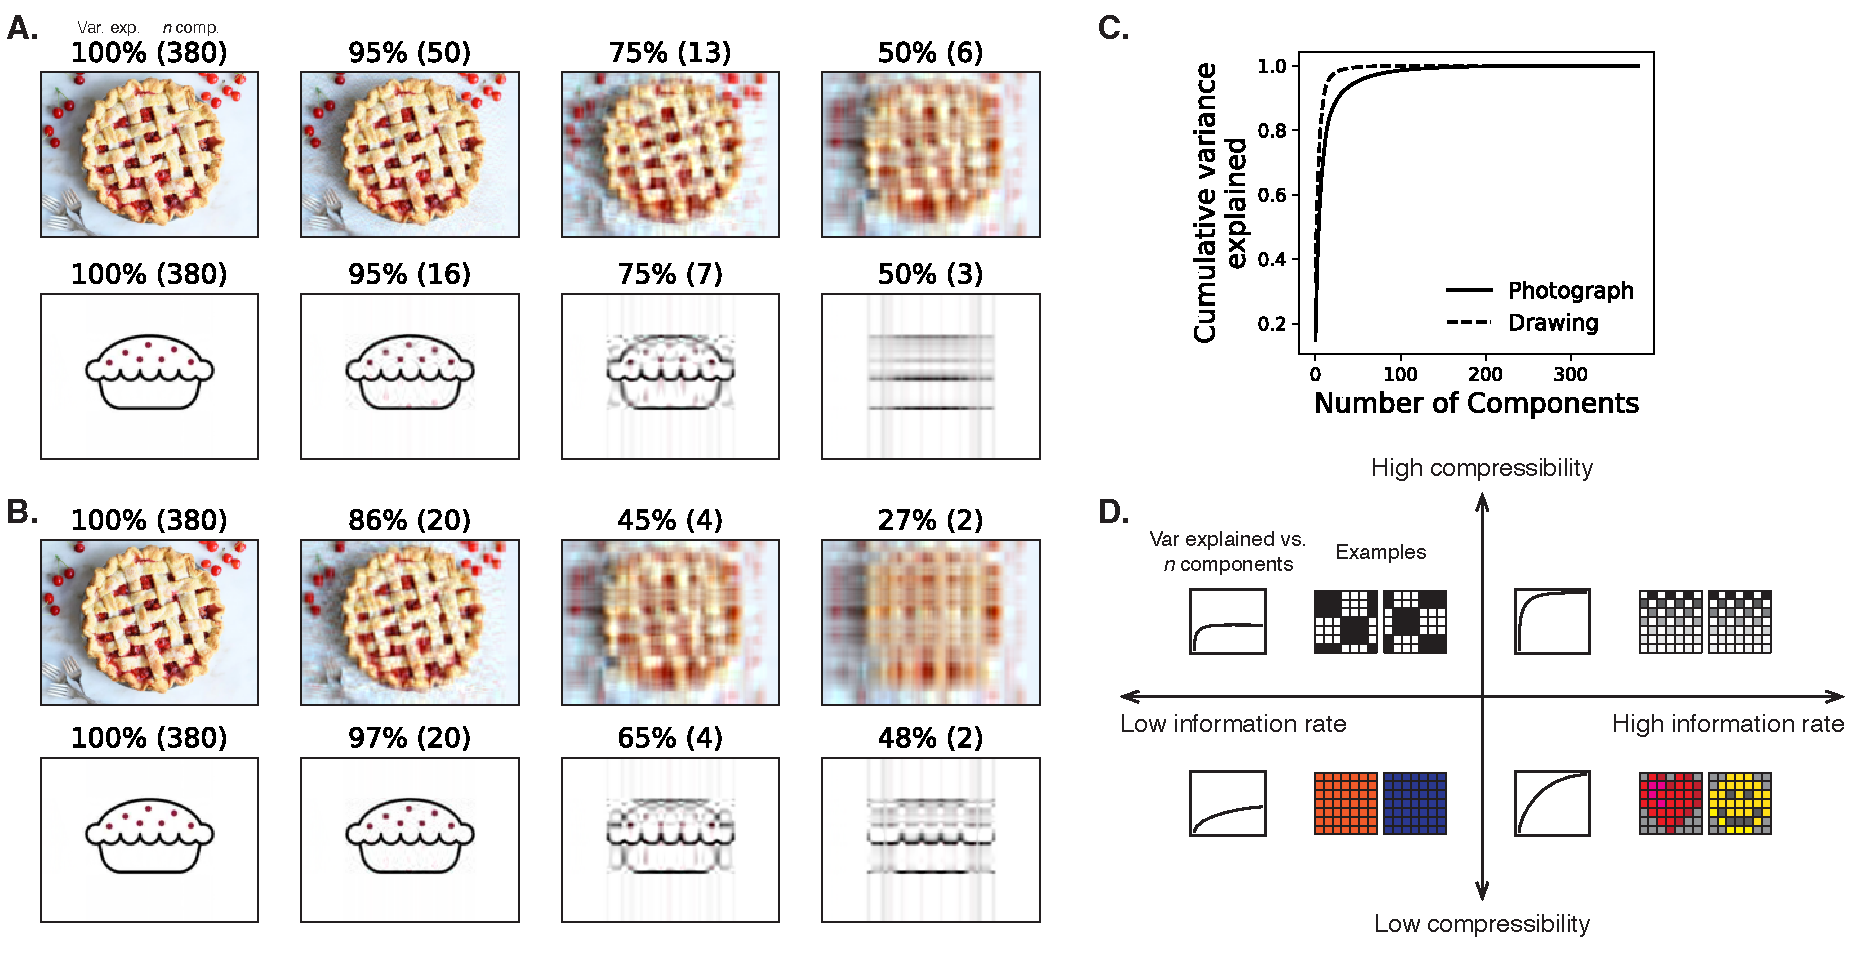
\includegraphics[width=\textwidth]{figs/information_and_compressibility}

\caption{\textbf{Information content and compressibility.} \textbf{A. Variance
explained for two images.} We applied principal components analysis to a
photograph and drawing, treating each row of the images as ``observations.''
Across columns, we identified the number of components required to explain
100\%, 95\%, 75\%, or 50\% of the cumulative variance in each image (the 100\%
columns denote the original images). The numbers of components are indicate in
parentheses, and the resulting ``compressed'' images are displayed. \textbf{B.
Representing two images with different numbers of components.} Using the same
principal component decompositions as in Panel A, we computed the cumulative
proportion of variance explained with 380 (original images), 20, 4, or 2
components. \textbf{C. Cumulative variance explained versus number of
components.} For the images displayed in Panels A and B, we plot the cumulative
proportion of variance explained as a function of the number of components used
to represent each image. \textbf{D. Information rate and compressibility.}
Across multiple images, the information rate (i.e., the amount of information
contained in each image; horizontal axis) is high when each individual pixel
provides information that cannot be inferred from other pixels.
High-information rate images tend to be high-resolution, and low-information
rate images tend to be low-resolution. Compressibility is related to the
difference between the information required to specify the original versus
compressed images (vertical axis). Highly compressible images often contain
predictable structure (redundancies) that can be leveraged to represent the
images much more efficiently than in their original feature spaces.}

\label{fig:information-compression} 
\end{figure}


% Specifically, if a given signal
% (e.g., a representation of brain activity patterns) contains more information
% about ongoing cognitive processes, then the peak decoding accuracy should be
% high. And if the signal is compressible, a low-dimensional embedding of the
% signal will be similarly informative to the original signal. A signal can be
% informative but not compressible, informative but




% %   - e.g., you could have something that is highly compressible (just a few components are sufficient to achieve some threshold information level) but
% %     *also* very rich-- e.g., the maximum number of informative components is large
% % compression and task demands -- MackEtal20, ZhouEtal19
% % superEEG -- prediction of held-out data; implies redundancy
% % timecorr -- higher order network patterns during higher order cognition implies more complexity
% % cognitive richness and scrambling-- various Hasson lab papers




% We're interested in the complexity of brain patterns that underly different
% types of thoughts. To explore this question space, we will take brain patterns
% recorded under different experimental conditions used in Aim 2, and project
% them into lower dimensional spaces using principle components analysis. We can
% then ask how well those low-dimensional embeddings of the data retain
% cognitively relevant information like when in a story someone is listening to.

% This work has been inspired, in part, by~\cite{MackEtal20}. In this paper, they
% investigated the role of the prefrontal cortex in filtering out irrelevant
% content. Specifically, they looked at if the vmPFC performs data reduction on
% incoming information through compression. This was motivated, in part, by
% orbital frontal cortex (OFC) compression in rats~\citep{ZhouEtal19}. They
% studied this using a learning paradigm in which participants had to classify
% insects based on different numbers of feature dimensions. The idea was that
% participants in some learning blocks, participants could identify the insects
% based on one feature (low complexity) or several features (high complexity),
% but importantly the stimuli remained the same across all learning problems.
% They found that complexity and compression had an inverse relationship; the
% lower complexity of a conceptual space, the higher the degree of compression.
% Building on this idea, we wonder if varying degrees of compression is performed
% throughout the brain. We also want to test this idea, but using varying levels
% of engagement listening to a naturalistic stimuli.

% To understand the degree of compression throughout the brain during cognition,
% we will use the same fMRI data from Aim 2, collected while participants
% listened to a story in different scrambling conditions. We will measure the
% degree that multivoxel activation patterns are compressed during story
% listening using principle components analysis (PCA) a method for low-rank
% approximation of multidimensional data~\citep{EckaYoun36}. We will explore this
% using decoding accuracy as a function of the number of components, or
% dimensions, in the low-dimensional space under different cognitive conditions.

% You can imagine two reasonable predictions of how cognition is reflected in
% brain patterns. The first is as our thoughts become more complex, they are
% supported by more complex brain patterns, and require more components to
% decode. The second is that when thoughts are deeper and more complicated, the
% units of neural activity would carry more information, and would require
% therefore fewer components to decode.


% This idea can be explored in this visual analogy (Fig.~\ref{fig: pie_example})
% for neural compression. Here there are two images of pies, the top pie is more
% complex than the bottom. On the left we're illustrating that it takes fewer
% components to reach the same 95 percent variance explained in the less complex
% pie, which corresponds to higher compression. However, on the right with very
% few components similar variance is explaining both pies.


% We investigated the dimensionality of neural patterns by training
% classifiers using more and more principle components. Or, in other
% words, we used less and less compression to decode.
% We applied the approach to
% a neuroimaging dataset comprising data collected as participants
% listened to a story varying in cognitive richness~\citep{SimoEtal16}.



% % PCA, or the closely related factor analysis and singular value decomposition (SVD) (Hastie et al., 2009), is widely used in the study of individual differences and aids estimating how many latent components, or “factors”, underlie a pattern of (item) responses within or across participants, as for instance in the context of intelligence (Spearman, 1904) or personality tests (Cattell, 1947). In the context of neuroimaging, PCA has been used to identify brain networks (Huth et al., 2012; Friston et al., 1993). 

%  % add citation:
% % S.M.Smith,A.Hyva ̈rinen,G.Varoquaux,K.L.Miller,and C. F. Beckmann, “Group-PCA for very large fMRI datasets,” NeuroImage, vol. 101, pp. 738, 2014.


% \subsection*{Evaluation metrics}
%  We will evaluate the degree of
% compression of held-out
% neuroimaging data by assessing the time at which it was collected.  We will use this evaluation (timepoint
% decoding) as a proxy for
% gauging how much explanatory power the compressed data held
% with respect to the observed data.



% \subsubsection*{Timepoint decoding}

% To explore how compression varies with complexity, we will use a previous neuroimaging dataset
% ~\cite{SimoEtal16}  in which participants listened to an audio recording of a story; 36 particpants listen to an intact version of the story, 17 participants listen to time-scrambled recordings of the same story where paragraphs were scrambled, 36 particpants listen to word-scrambled version and 36 participants lay in rest condition.


% Following the analyses conducted by (HTFA)~\cite{MannEtal18}, we first
% apply \textit{hierarchical topographic factor analysis} (HTFA) to
% the fMRI datasets to obtain a time series of 700 node activities for
% every participant.  We then apply dimensionality reduction
% (Incremental PCA) for each group.

% We then compare the groups’ activity patterns (using Pearson
% correlations) to estimate the story times each corresponding pattern
% using more and more principle components.   

% To assess decoding accuracy, we randomly divide participants for each
% stimulus into training and testing groups. We then compare the
% groups’ activity patterns (using Pearson correlations) to estimate the
% story times each corresponding pattern using more and more principle
% components (as the data became less compressed). Specifically, we ask, for each timepoint: what are the correlations
% between the first group's and second group's activity patterns at each
% order. We note that the decoding test we used is a conservative in which we count a timepoint label as incorrect if it is not an exact match.





% \subsection*{Evaluation metrics}
%  We evaluated the degree of
% compression of held-out
% neuroimaging data with the time at which it was collected.  We used this latter evaluations (using timepoint
% decoding) as a proxy for
% gauging how much explanatory power the compressed data held
% with respect to the observed data.



% \subsubsection*{Timepoint decoding}

% To explore how higher-order structure varies with stimulus structure
% and complexity, we used a previous neuroimaging dataset
% ~\cite{SimoEtal16}  in which participants listened to an audio recording of a story; 36 particpants listen to an intact version of the story, 17 participants listen to time-scrambled recordings of the same story where paragraphs were scrambled, 36 particpants listen to word-scrambled version and 36 participants lay in rest condition.

% Prior work has shown participants share similar neural responses to
% richly structured stimuli when compared to stimuli with less
% structure.  To assess whether the moment-by-moment higher order
% correlations were reliably preserved across participants, we used
% inter-subject functional connectivity (ISFC) to isolate the
% time-varying correlational structure (functional connectivity patterns
% that were specifically driven by the story participants listened to.
% Following the analyses conducted by (HTFA)~\cite{MannEtal18}, we first
% applied \textit{hierarchical topographic factor analysis} (HTFA) to
% the fMRI datasets to obtain a time series of 700 node activities for
% every participant.  We then applied dimensionality reduction
% (Incremental PCA) for each group.

% We then compared the groups’ activity patterns (using Pearson
% correlations) to estimate the story times each corresponding pattern
% using more and more principle components.   

% To assess decoding accuracy, we randomly divided participants for each
% stimulus into training and testing groups. We then compared the
% groups’ activity patterns (using Pearson correlations) to estimate the
% story times each corresponding pattern using more and more principle
% components (as the data became less compressed). Specifically, we asked, for each timepoint: what are the correlations
% between the first group's and second group's activity patterns at each
% order. We note that the decoding test we used is a conservative in which we count a timepoint label as incorrect if it is not an exact match.



\section*{Results}
By training classifiers using more and more principle components to decode, and comparing across conditions with varying degrees of cognitive richness, we can assess the explanatory power of the compressed data held with respect to the observed data (see \textit{Methods}). We note that our primary goal was not to achieve perfect decoding accuracy, but rather to use decoding accuracy as a benchmark for assessing whether different neural features specifically capture cognitively relevant brain patterns.

\begin{figure}
  \centering
  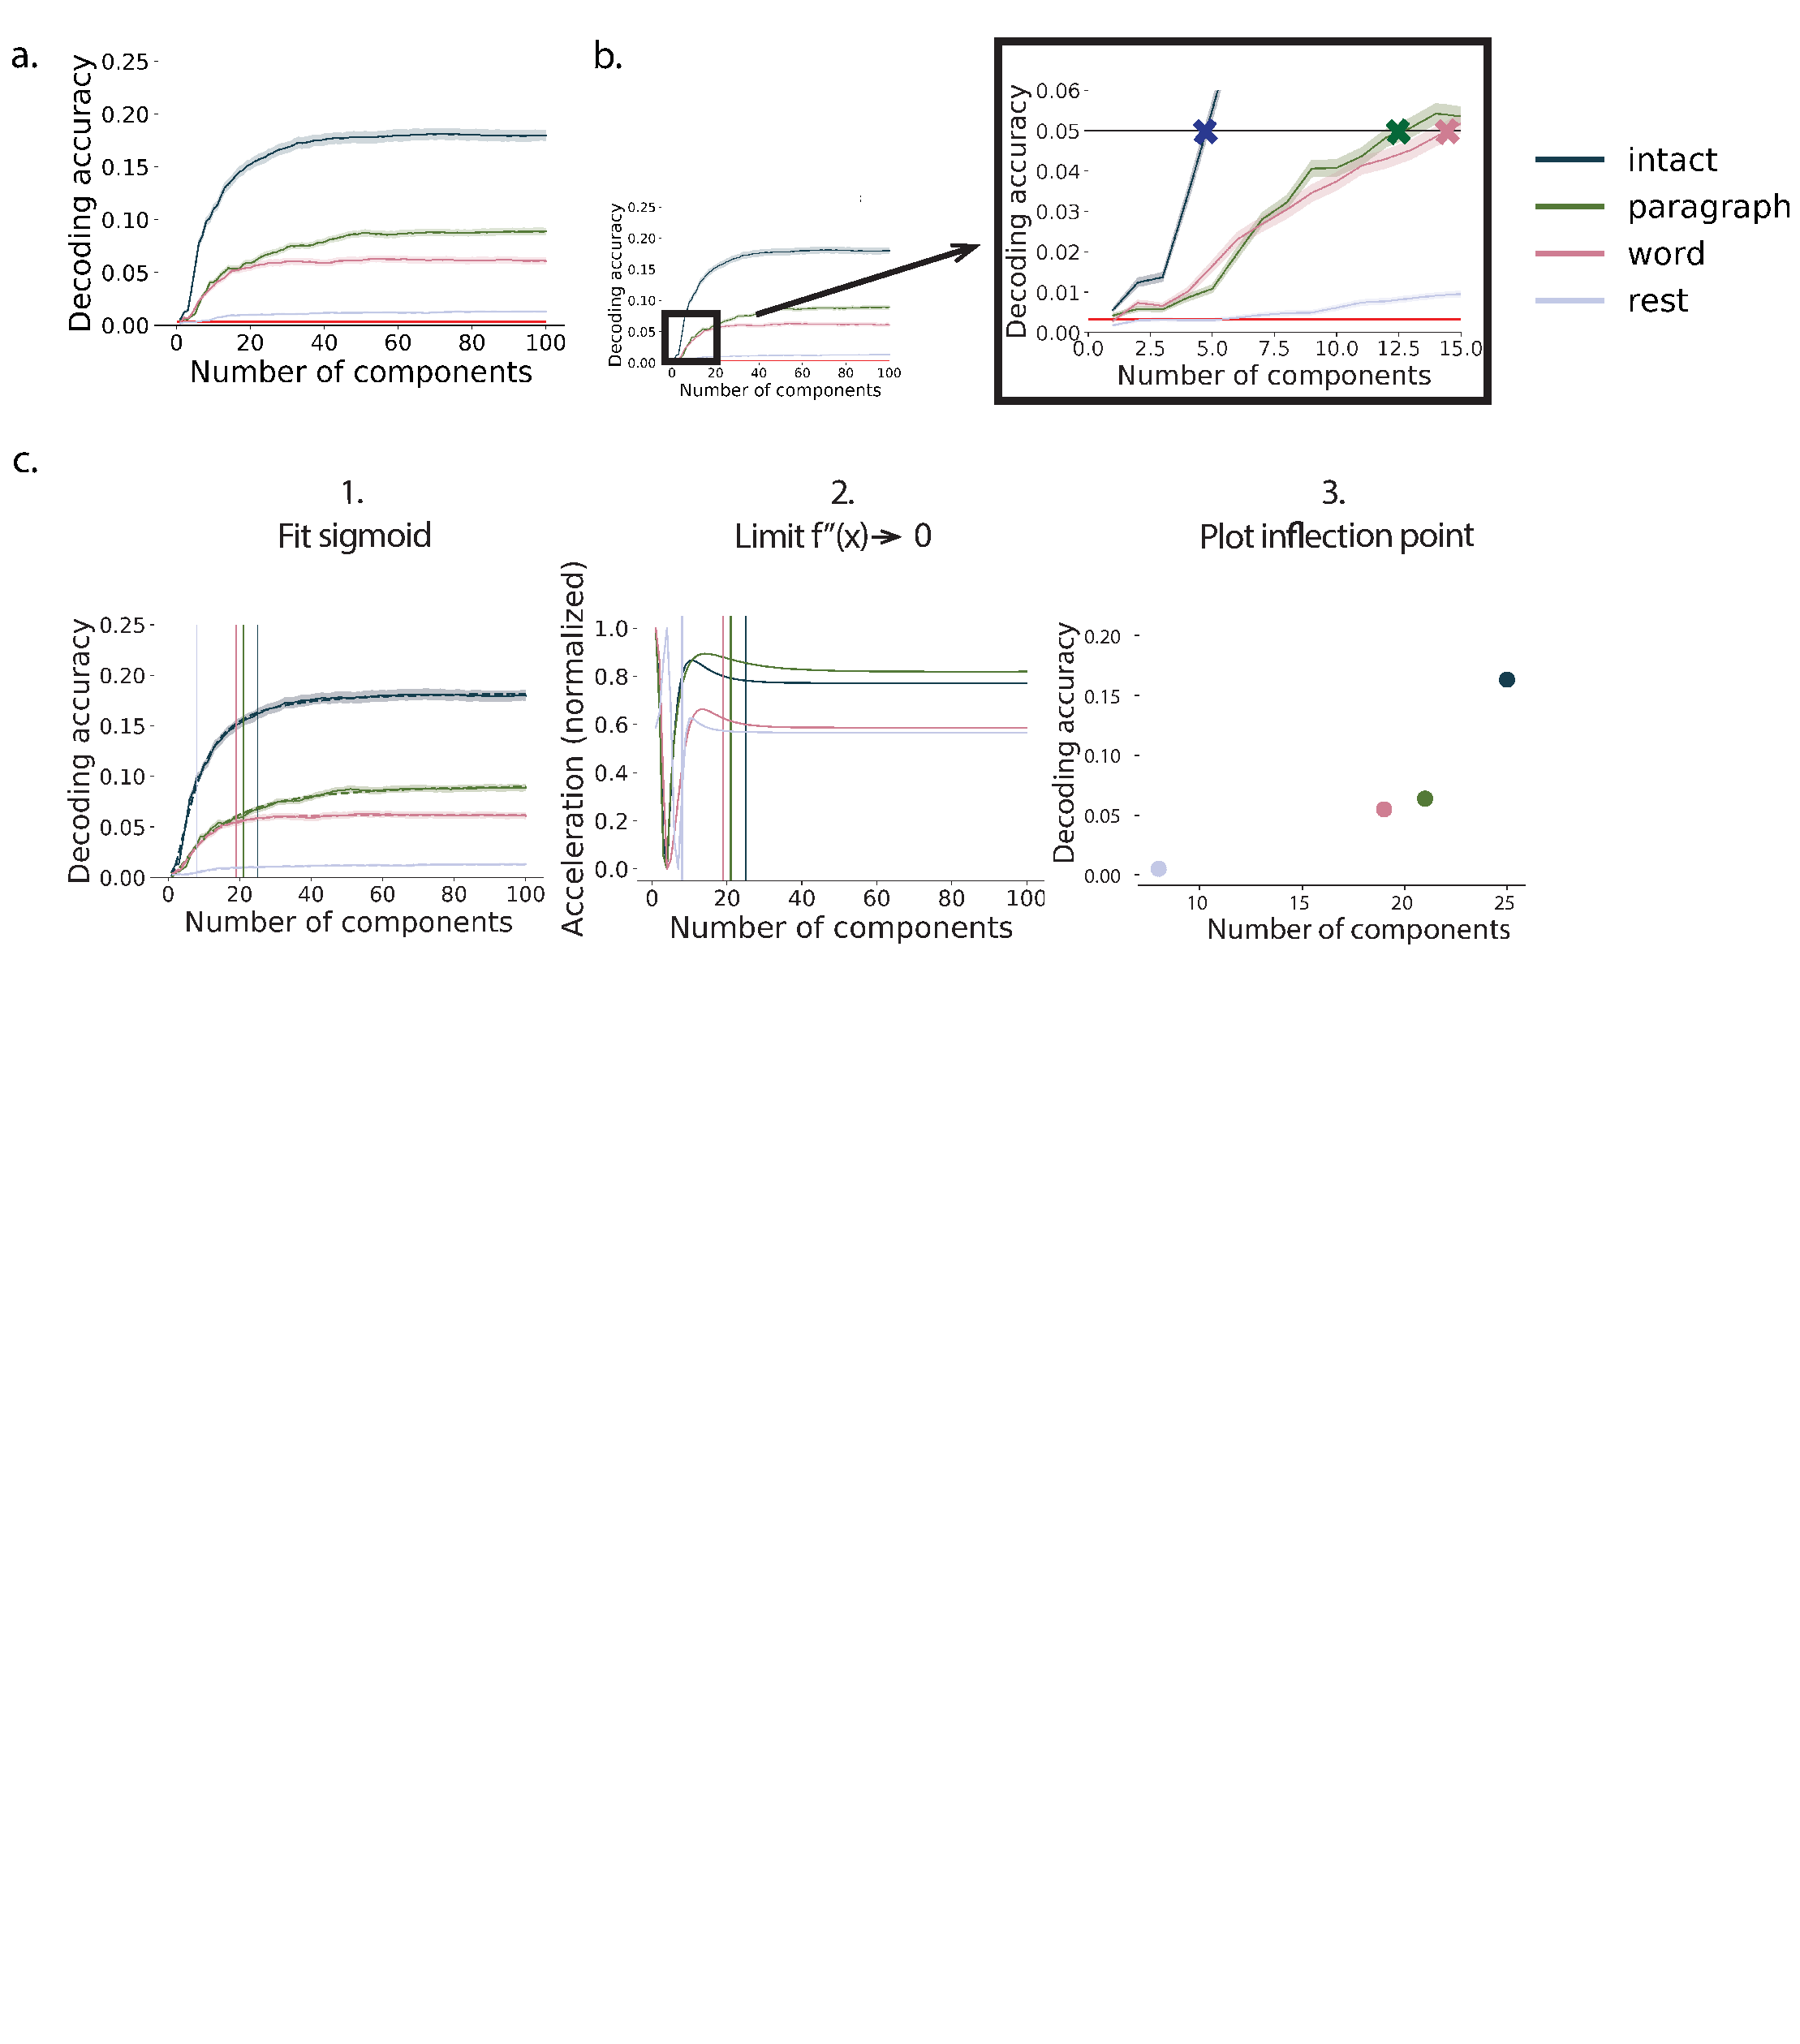
\includegraphics[width=\textwidth]{figs/decode_interpret.pdf}
  \caption{\textbf{Decoding accuracy.} \textbf{a. Decoding accuracy by
      number of components.} Ribbons of each color display
    cross-validated decoding performance for each condition (intact,
    paragraph, word, and rest). Decoders were trained using
    increasingly more principle components and displayed relative to
    chance (red line). \textbf{b. Fixed decoding accuracy by number of
      components.} We zoom in on the plot shown in \textbf{a.} and add
    a line denoting fixed decoding accuracy (.05). We plot where the
    intact, paragraph, and word conditions intersect.
    \textbf{c. Explanation of inflection metric.} First the we fit a sigmoid function to the decoding accuracy by number of components. Second, we found where the second derivative is both positive and less than .0001. Last, we then plot that inflection point as a single metric to capture the slope and asymptote of the curve.}
    \label{fig:decode_interpret}
  \end{figure}



Prior work has shown participants share similar neural responses to
richly structured stimuli when compared to stimuli with less
structure \cite{SimoEtal16}.  We replicate this finding, showing as complexity of the stimulus increases, decoding accuracy
increases (Fig.~\ref{fig:decode_interpret},  a.).  
Additionally, we found that as complexity of the stimuli increases, we need fewer components to decode the same amount (Fig.~\ref{fig:decode_interpret},  b.). However, we also found that as complexity of the stimuli increases, more components are required to reach peak decoding accuracy (Fig.~\ref{fig:decode_interpret},  c.).  
We posit that as the complexity of our thoughts increases, neural
compression decreases. However, as our thoughts become deeper and richer, more reliable information is available at higher neural compression.



% We performed a decoding analysis, using cross validation to estimate
% (using other participants’ data) which parts of the story the additional added
% principle component corresponded to (see \textit{Materials and methods}). We note that our primary goal was not to achieve perfect decoding accuracy, but rather to use decoding accuracy as a benchmark for assessing whether different neural features specifically capture cognitively relevant brain patterns.

% Separately for each experimental condition, we divided participants
% into two groups. Starting with 1 principle comonent, for
% each dimension we added another principle component, and we correlated the group 1 activity patterns with group 2
% activity patterns.  There were 272
% timepoints for paragraph condition, 300 timepoints for intact and word
% conditions, and 400 timepoints for rest condition,  so chance
% performance on this decoding test is was $\frac{1}{272}$,
% $\frac{1}{300}$, and $\frac{1}{400}$ respectively.
 
% - As complexity of the stimulus increases, decoding accuracy
% increases (Fig.~\ref{fig:decode_interpret},  a.).  Replication of
% Simony findings. 

% - As complexity of the stimuli increases, we need fewer components to
% decode the same amount (Fig.~\ref{fig:decode_interpret},  b.).  

% - As complexity of the stimuli increases, more components are required to reach peak decoding accuracy (Fig.~\ref{fig:decode_interpret},  c.).  

\begin{figure}
  \centering
  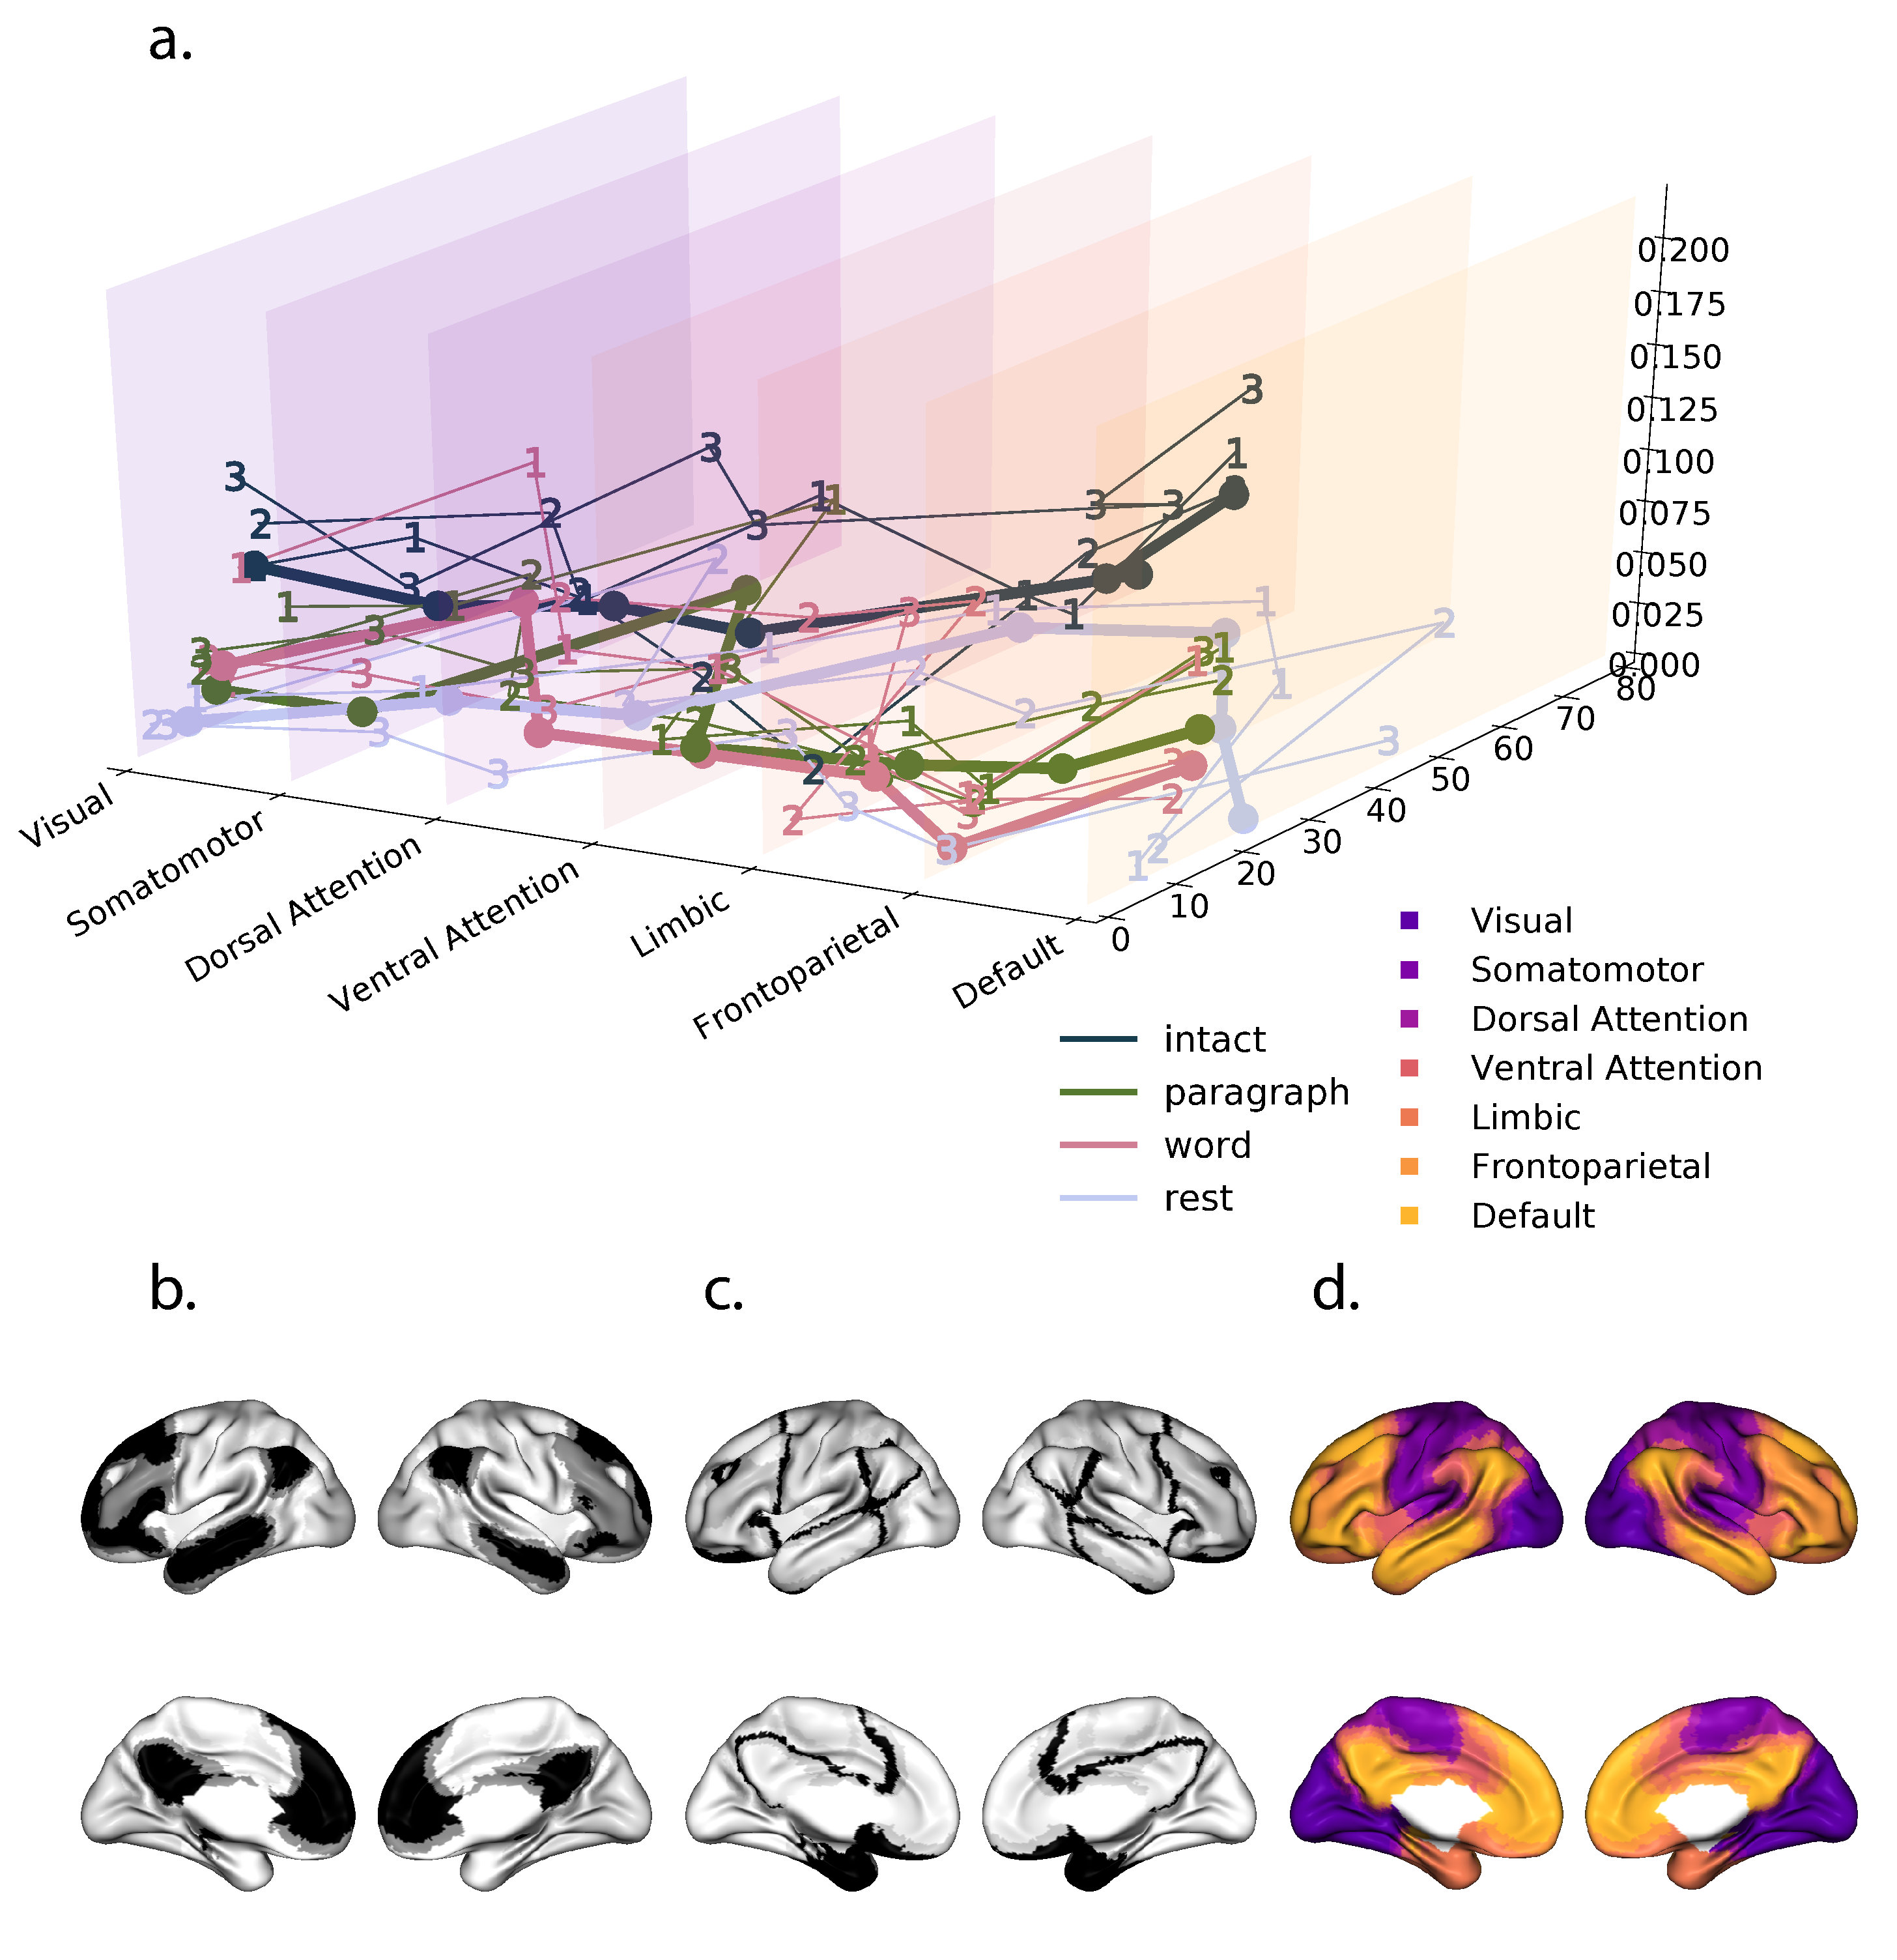
\includegraphics[width=\textwidth]{figs/decode_pcs_network.pdf}
  \caption{\textbf{Inflection points by network.} \textbf{a.}
    Inflection point was calculated as explained in
    Fig.~\ref{fig:decode_interpret}, b. Analyses were limited by the
    brain networks (using the \cite{YeoEtal11} network parcellation) and
    arranged in increasing order relative to the intact condition.
    \textbf{b. and c.} For the total time in the intact condition, we are plotting the relative inflection points (\textbf{b.}) and corresponding number of components (\textbf{c.}) by network. \textbf{d.} The network parcellation defined by \cite{YeoEtal11} is displayed on the inflated brain maps. The colors and network labels serve as a legend for \textbf{a.} and \textbf{d.}}
  \label{fig:decode_pcs_network}
\end{figure}

We also wondered how this compression would change across brain regions.  We repeated the analysis but limited the brain hubs to 7 networks using the Yeo et al. (2011) network parcellation shown here in the inflated brain (Fig.~\ref{fig:decode_pcs_network}, d.). We found that as complexity of the stimuli increases, decoding accuracy increases
with higher cognitive areas. (Fig.~\ref{fig:decode_pcs_network}).


% As complexity of the stimuli increases, decoding accuracy increases
% with higher cognitive areas. (Fig.~\ref{fig: decode_pcs_network}).

%  If, there is some understanding of the narrative that accumulates over time, we should be able to see that change.

\begin{figure}
  \centering
  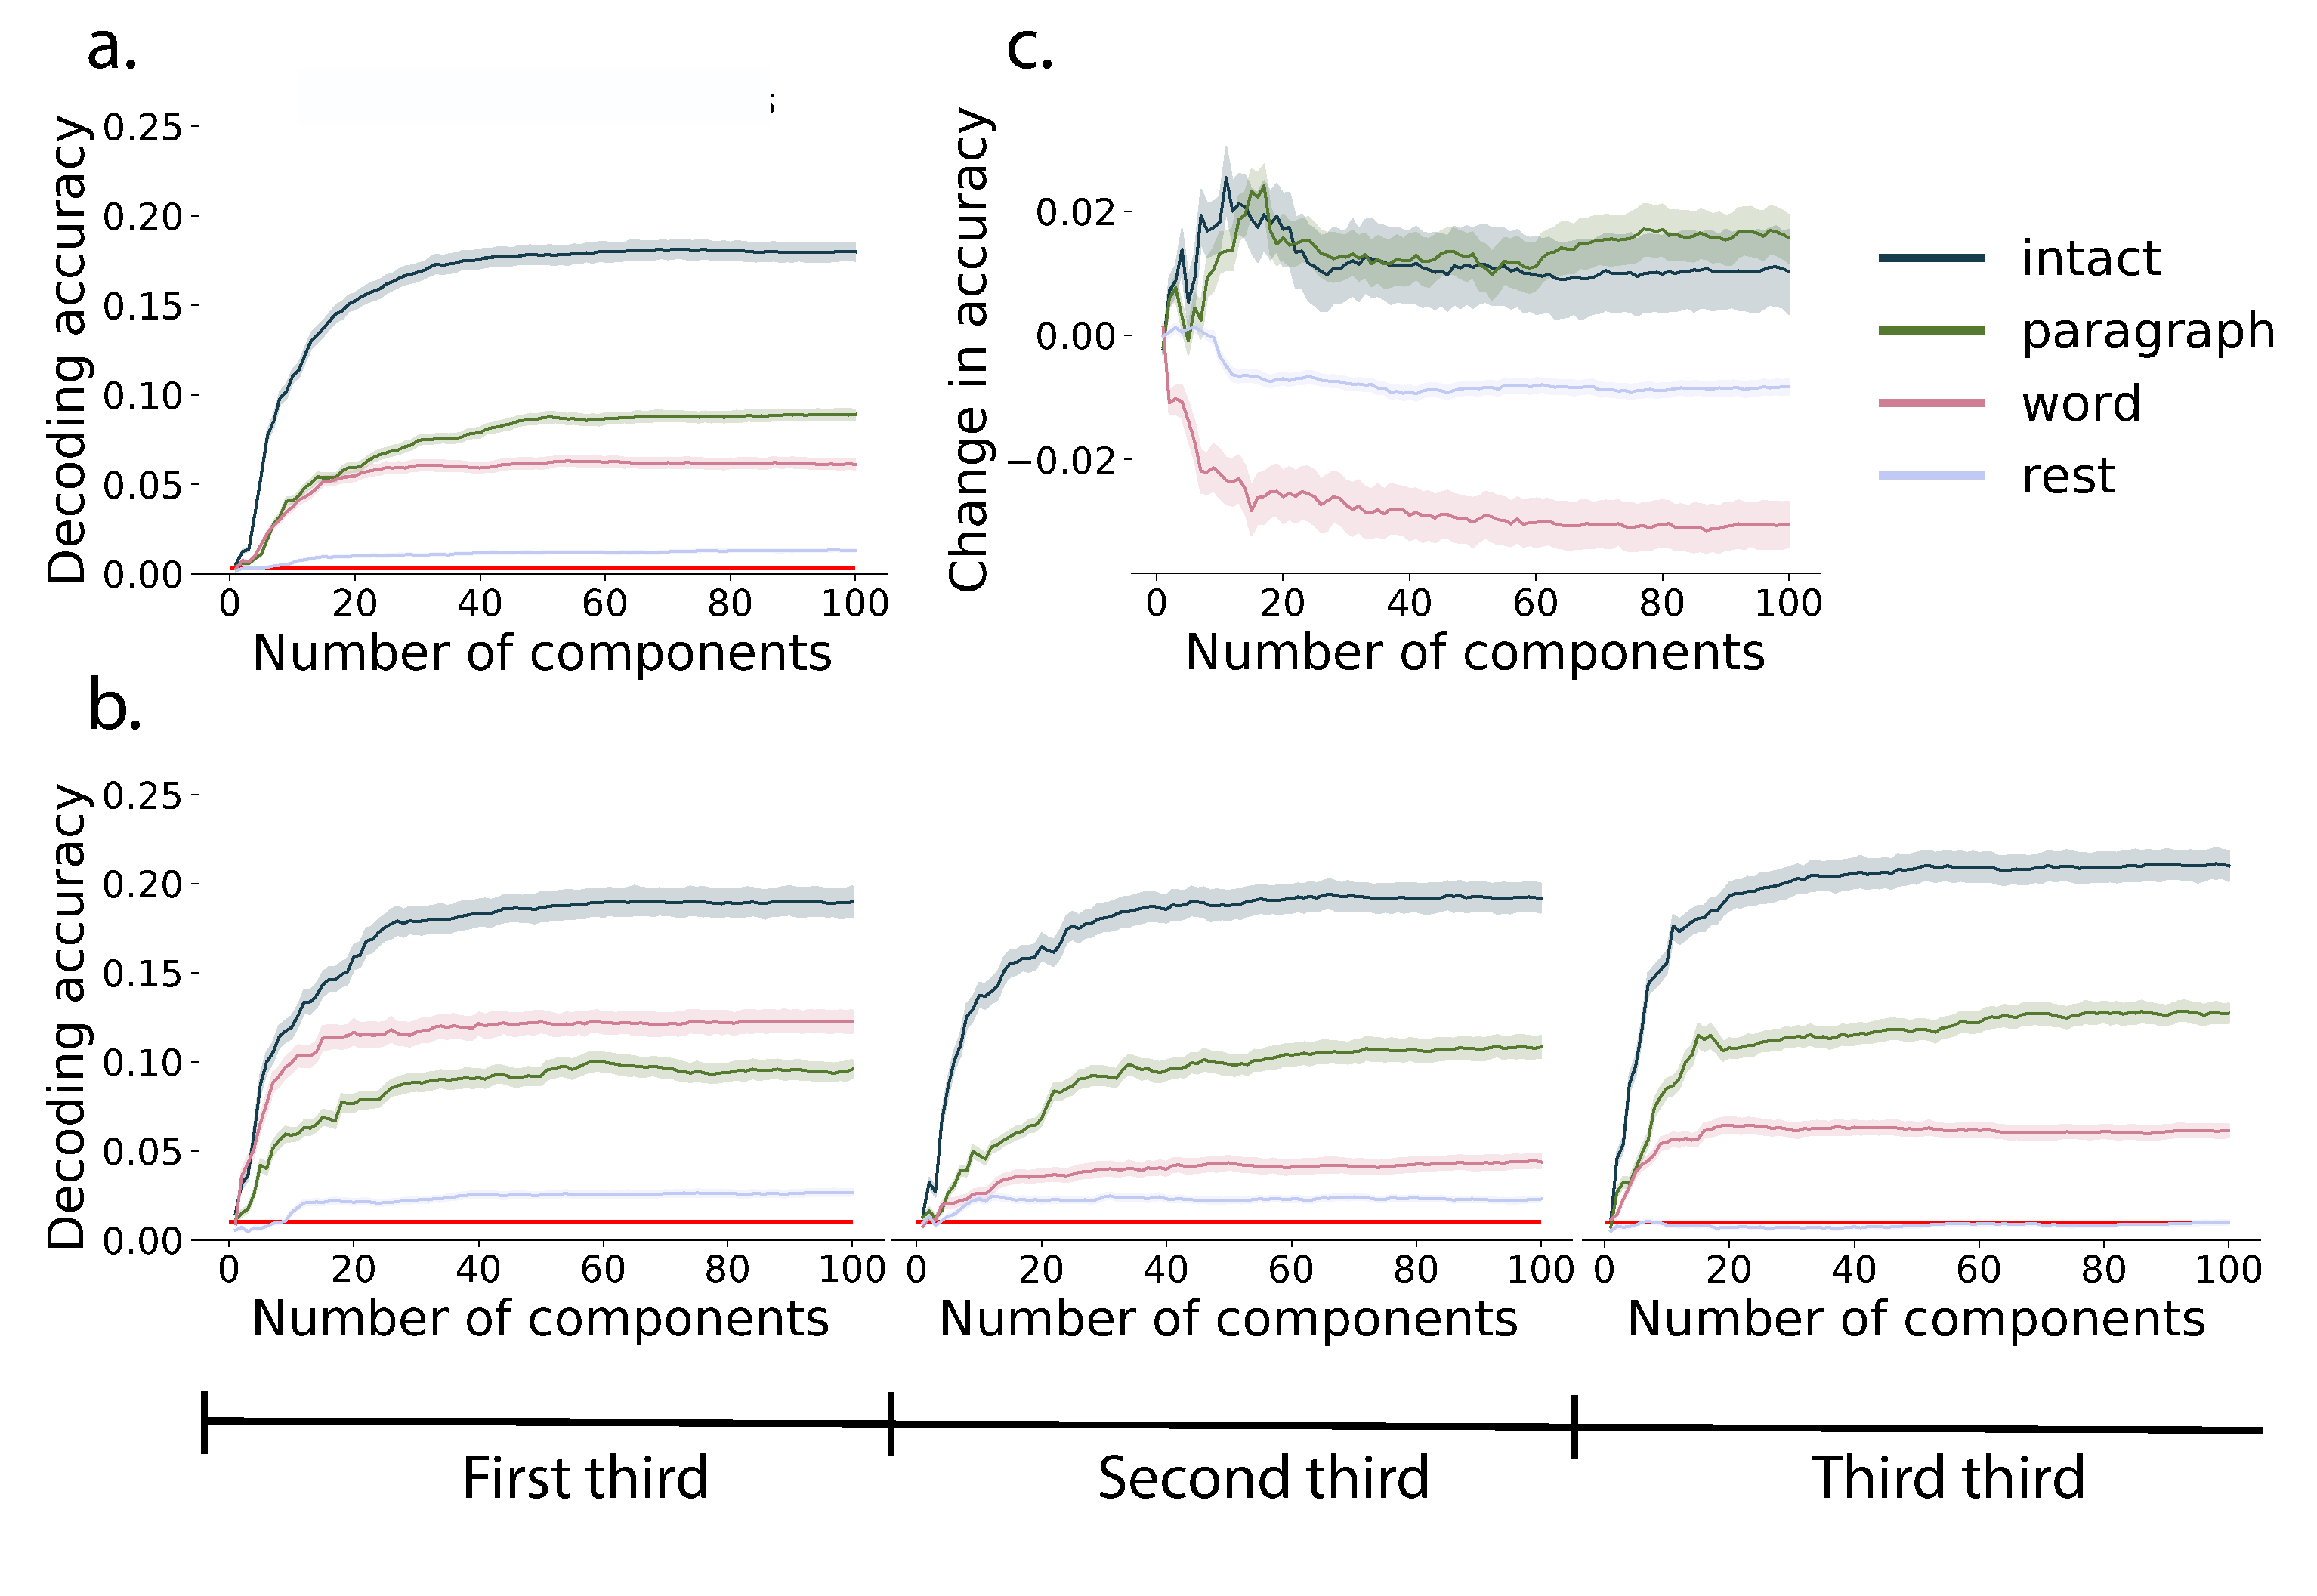
\includegraphics[width=\textwidth]{figs/decode_pcs.pdf}
  \caption{\textbf{Inflection points by thirds.} \textbf{a.}
    Decoding accuracy by number of components not broken into thirds
    (Fig.~\ref{fig:decode_interpret} a.). \textbf{b. and c.}
    Quantifying changes in decoding accuracy across
time. \textbf{b.} Slope of decoding accuracy was calculated by fitting
a regression line for each component/condition for each
third. \textbf{c.}  We also repeated the analysis
(Fig.~\ref{fig:decode_interpret}, b.) to obtain the inflection point
for each condition and for each third. \textbf{d.}  Decoding accuracy by number of components for each third of the scan time. We repeated the same analysis in Fig.~\ref{fig:decode_interpret} a. but breaking the scan time for each condition into 3 intervals.
}
  \label{fig:decode_pcs_thirds}
\end{figure}

We were also curious how compression would change across time.  If, there is some understanding of the narrative that accumulates over time, we should be able to see that difference. We found increases in decoding accuracy with the same number or fewer components for more complex, cognitively rich, conditions.
We also found decreases in decoding accuracy for the word-scrambled and rest
condition.

Overall, we found that as story listening conditions become more complex, more components are required to decode. We also found we could decode better with more impoverished data when
there is the underlying structure of the narrative providing more cognitive richness. We posit that as the complexity of our thoughts increases, neural compression decreases. However, as our thoughts become deeper and richer, more reliable information is available at higher neural compression.



% - Increases in decoding accuracy with the same number or fewer components for more complex, cognitively rich, conditions.
% - Decreases in decoding accuracy for the word-scrambled and rest
% condition.


%%%%%%%%%%%%%%%%%%%%%%%%%%%%%%%%%%%%%%%
\section*{Discussion}


- We trained classifiers using more and more principle components to decode, and compared across condi- tions with varying degrees of cognitive richness.
-We found that as listening conditions become more cognitively rich,
decoding accuracy increased.
-Also, decoding accuracy increased as understanding of the narrative
accumulated over time, in more complex listening conditions.
- Decoding accuracy also increased in higher cognitive areas, in more complex listening conditions.
-We found that as story listening conditions become more complex, more
components are required to decode.
-We also found we could decode better with more impoverished data when
there is the underlying structure of the narrative providing more cognitive richness.
-We posit that as the complexity of our thoughts increases, neural
compression decreases. However, as our thoughts become deeper and richer, more reliable information is available at higher neural compression.







Based on prior work ~\citep{Deme19} and following the direction of the field ~\citep{Turk13} we think our thoughts might be encoded in
dynamic network patterns, and possibly higher order network
patterns (Fig.~\ref{fig:direction_of_field}). We sought to test this hypothesis by developing an approach
to inferring high-order network dynamics from timeseries data. 

One challenge in studying dynamic interactions is the
computational resources required to calculate higher-order correlations. 
We developed a computationally tractable model of network dynamics (Fig.~\ref{fig:methods_fig}) that takes in a feature
timeseries and outputs approximated first-order dynamics (i.e.,
dynamic functional correlations), second-order dynamics
(reflecting homologous networks that dynamically form and disperse),
and higher-order network dynamics (up to tenth-order dynamic
correlations).

We first validated our model using synthetic data, and explored how
recovery varied with different underlying data structures and kernels.   We then 
applied the approach to an fMRI dataset
~\citep{SimoEtal16} in which participants listened to an audio
recording of a story, as well as scrambled versions of the same story
(where the scrambling was applied at different temporal scales).  We
trained classifiers to take the output of the model and decode the
timepoint in the story (or scrambled story) that the participants were
listening to. We found that, during the intact listening condition in the
experiment, classifiers that incorporated higher-order correlations
yielded consistently higher accuracy than classifiers trained only on
lower-order patterns (Fig.~\ref{fig:decoding_level},  a.\&d.).  By contrast, these
higher-order correlations were not necessary to support decoding the other
listening conditions and (minimally
above chance) during a control rest condition.  This suggests
that the cognitive processing that supported the most cogntively rich listening conditions
involved second-order (or higher) network dynamics.

Although we found decoding accuracy was best when incorporating
higher-order network dynamics for all but rest
  condition, it is unclear if this is a product of the brain or the
  data collection technique.  It could be that the brain is
  second-order or it could be that fMRI can
  only reliably give second-order interactions. Exploring this method
  with other data collection technique will be important to
  disentangle this question.



  \subsection*{Concluding remarks}

How can we better understand how brain patterns change over
time? How can we quantify the potential network dynamics that might be
driving these changes? One way to judge the techniques of the future is
to look at the trajectory of the fMRI field so far has taken so far
(Fig.~\ref{fig:methods_fig}).  The field started with 
univariate activation, measuring the average activity for each voxel.
Analyses of multivariate activation followed, looking at spatial patterns of
activity over voxels. Next, correlations of activity were explored, first
with measures like resting connectivity that take temporal correlation
between a seed voxel and all other voxels then with full connectivty
that measure all pairwise correlations.  Additionally, this path of increasing
complexity also moved from static to dynamic measurements.  One
logical next step in this trajectory would be dynamic higher-order
correlations. We have created a method 
to support these calculations by scalably approximating dynamic higher-order
correlations.  

\section*{Acknowledgements}
We acknowledge discussions with Luke Chang, Hany Farid, Paxton
Fitzpatrick, Andrew Heusser, Eshin Jolly, Qiang Liu, Matthijs van der
Meer, Judith Mildner, Gina Notaro, Stephen Satterthwaite, Emily
Whitaker, Weizhen Xie, and Kirsten Ziman. Our work was supported in
part by NSF EPSCoR Award Number 1632738 to J.R.M. and by a sub-award
of DARPA RAM Cooperative Agreement N66001-14-2-4-032 to J.R.M.  The
content is solely the responsibility of the authors and does not
necessarily represent the official views of our supporting
organizations.

\section*{Author contributions}
Concept: J.R.M. and L.L.W.O. Implementation: L.L.W.O., and
J.R.M.  Analyses: L.L.W.O and J.R.M.

\bibliographystyle{apacite}
\bibliography{CDL-bibliography/cdl}

\end{document}


